
\begin{frame}

\'Elément principal de la réécriture nominal : pattern matching. Indique si un
terme est de la forme d'un \emph{pattern} (motif) donné, et en extrait des informations

\bigskip

Deux types de pattern matching : 
\begin{itemize}
\item Linéaire. 
\item Non linéaire. 
\end{itemize}

\end{frame}

\subsection{Pattern matching linéaire}


\begin{frame}
\frametitle{Exemple de pattern matching}

Prenons ce terme :
\texttt{Lambda(x, Var(x))}. 
\begin{itemize} 

  \item matche \texttt{Lambda(\_, \_)}.
  \item mais pas \texttt{Var(\_)}.

\end{itemize}

\bigskip

Extraction de sous-termes :

\texttt{Lambda(?x, \_)} retourne le sous-terme correspondant à \emph{?x}.

\end{frame}

\begin{frame}
\frametitle{Concrètement}

Exemple du déroulement du pattern-matching:
\begin{itemize}
  
  \item Terme : \texttt{Lambda(y, Var(y))}.

  \item Pattern : \texttt{Lambda(\_, Var(?x))}.

\end{itemize}

\bigskip

\begin{center}
  \only<2>
      {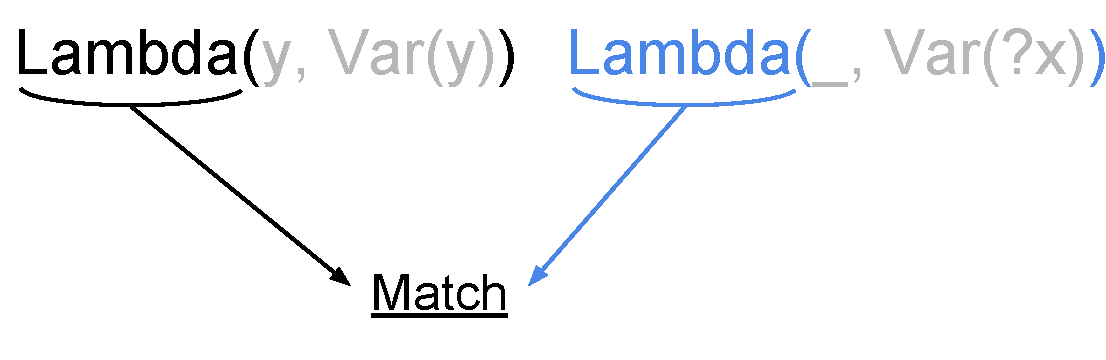
\includegraphics[scale=0.5]{pattern/trivial1.pdf}}
  \only<3>
      {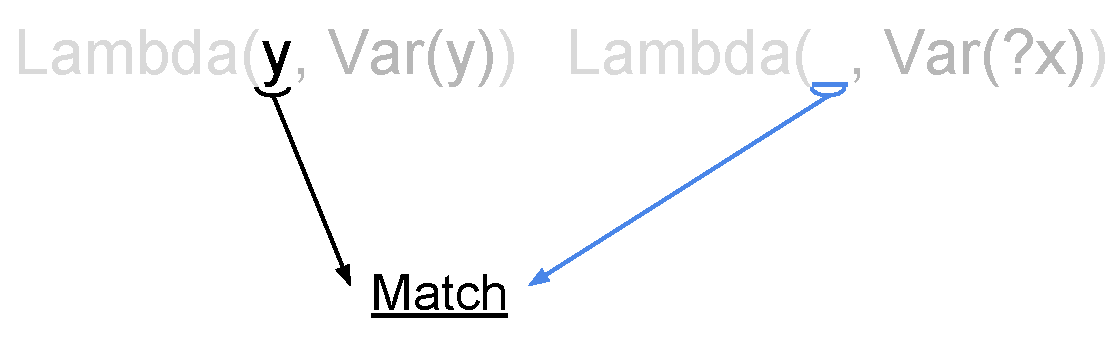
\includegraphics[scale=0.5]{pattern/trivial2.pdf}}
  \only<4>
      {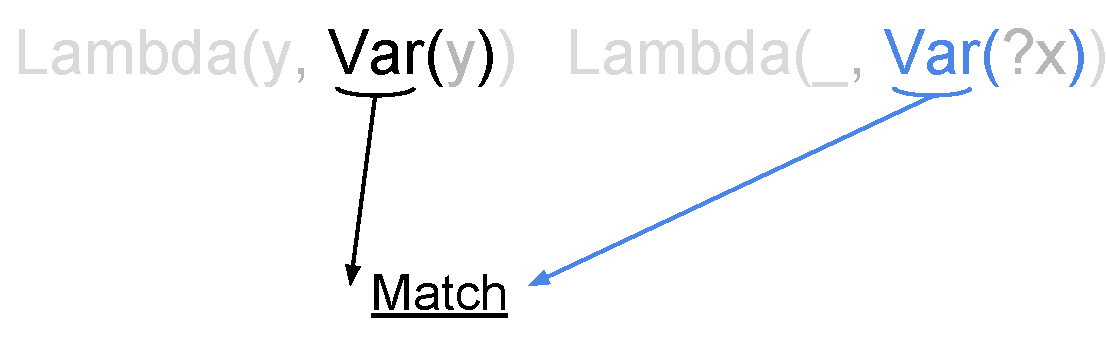
\includegraphics[scale=0.5]{pattern/trivial3.pdf}}
  \only<5>
      {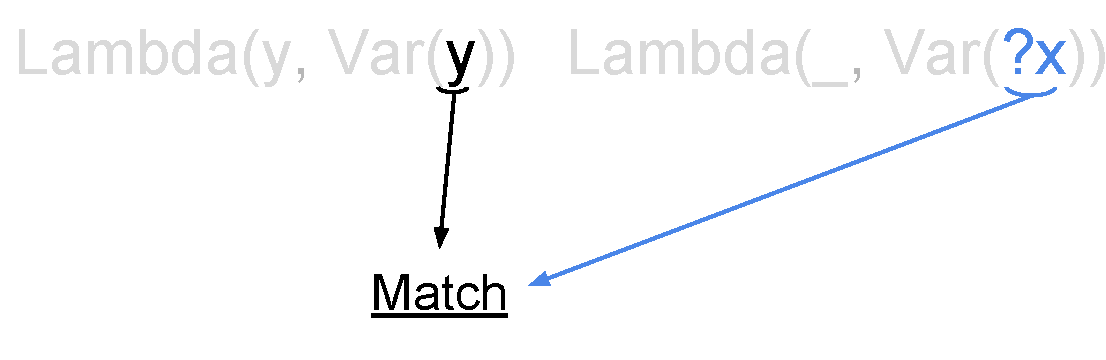
\includegraphics[scale=0.5]{pattern/trivial4.pdf}}
  \only<6>
      {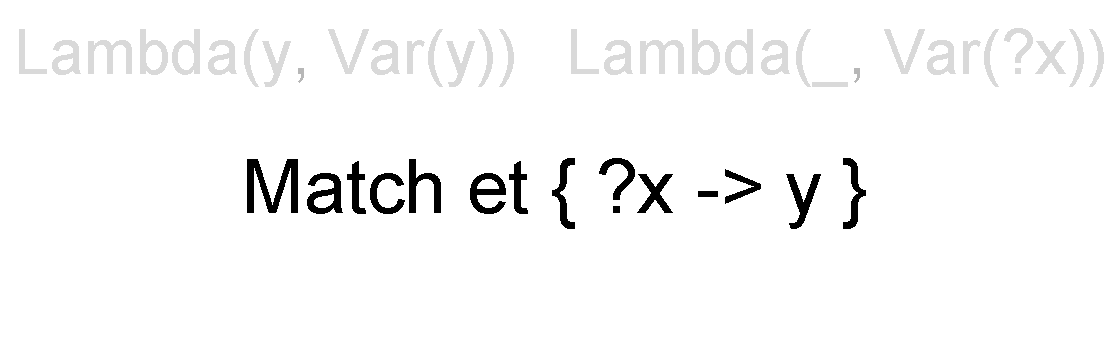
\includegraphics[scale=0.5]{pattern/trivial5.pdf}}

\end{center}

\end{frame}

\begin{frame}
\frametitle{Non linéarité des atomes}

Possibilité de matcher deux atomes liés même dans le cas linéaire.

Par exemple avec \texttt{Lambda(?x, Var(?x))} :

\bigskip
\begin{center}
  \only<2>
      {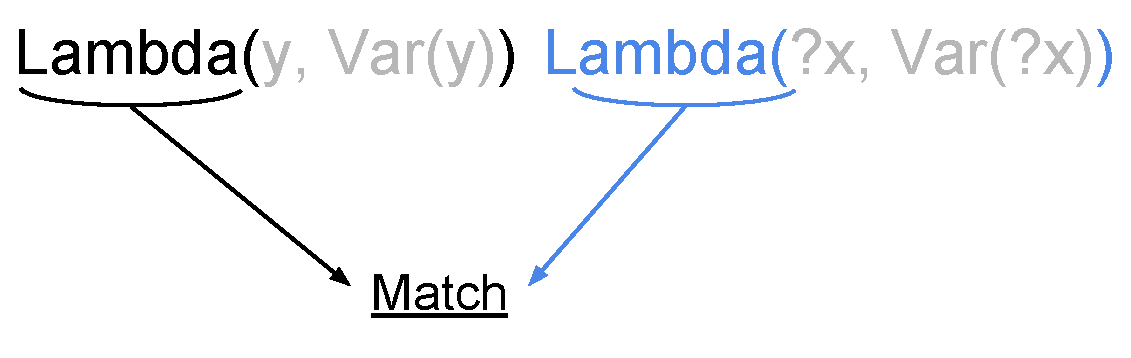
\includegraphics[scale=0.5]{pattern/atom1.pdf}}
  \only<3>
      {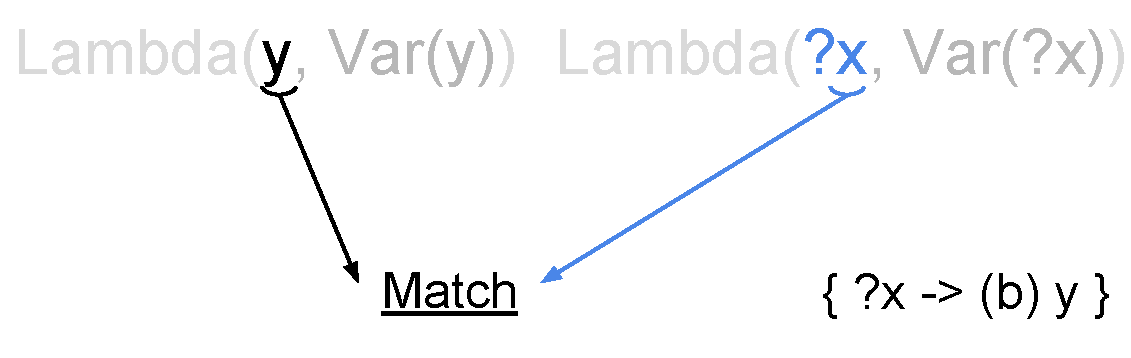
\includegraphics[scale=0.5]{pattern/atom2.pdf}}
  \only<4>
      {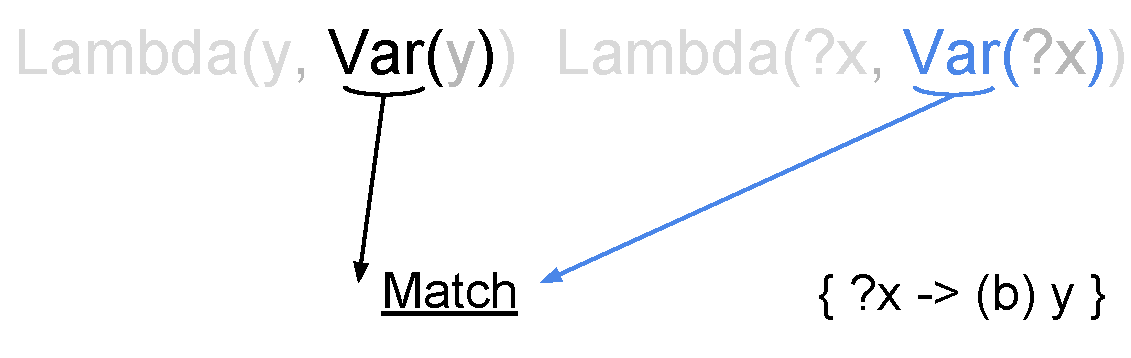
\includegraphics[scale=0.5]{pattern/atom3.pdf}}
  \only<5>
      {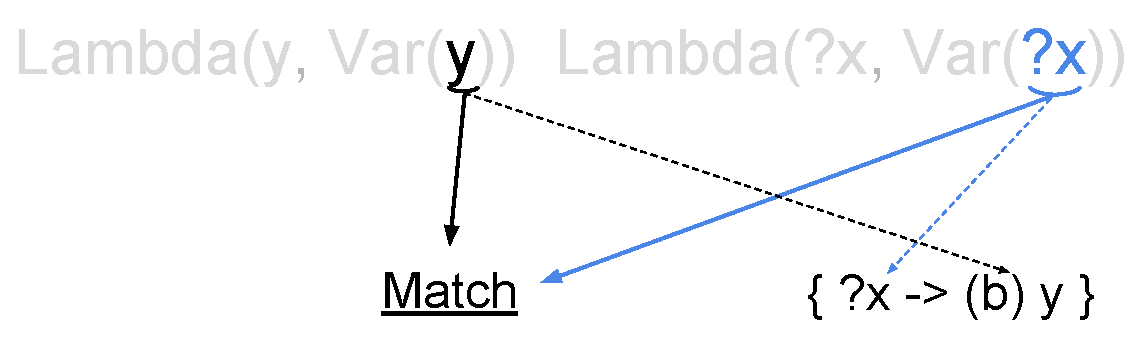
\includegraphics[scale=0.5]{pattern/atom4.pdf}}
  \only<6>
      {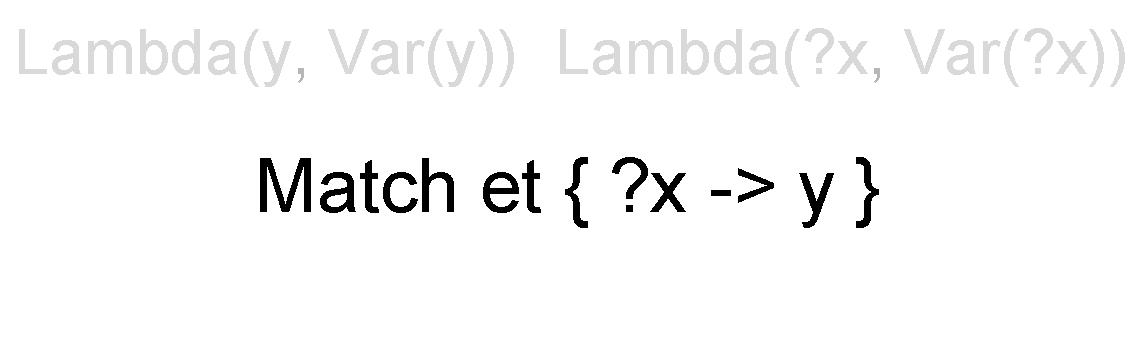
\includegraphics[scale=0.5]{pattern/atom5.pdf}}

\end{center}


\end{frame}

\subsection{Pattern matching non linéaire}

\begin{frame}
\frametitle{Non linéarité avec les termes}

Non linéarité : possiblité d'extraire plusieurs fois le même motif modulo
alpha-conversion.
\begin{itemize}
\item Atomes : possible dans l'algorithme linéaire.
\item Termes : nécessite la capacité de raisonner sur la structure du terme.
\end{itemize}

\bigskip

Exemple :
\begin{itemize}
\item Terme : \texttt{App(Lambda(x, Var(x)), Lambda(y, Var(y)))} matche 
\item Pattern : \texttt{App(?X, ?X)}.
\end{itemize} 

\medskip

Possible puisque le Lambda de droite n'est qu'un renommage du
Lambda de gauche.

\end{frame}

\begin{frame}
\frametitle{Solution : hashconsing}

Une solution élégante permet de régler ce problème : le hashconsing. 

Principe du hashconsing : ne pas allouer deux fois deux structures
identiques. 

\medskip

$\Rightarrow$ Deux termes structurellement identiques seront
le même objet alloué en mémoire.

\bigskip

Le hashconsing des termes fait abstraction des noms de binders et de variables
liées.

\end{frame}

\begin{frame}[fragile]
\frametitle{Hashconsing : exemple d'égalité structurelle}

\begin{columns}
  \column{.5\textwidth}
  Pour le terme 
  \begin{verbatim}
  App(
     Lambda(x, Var(x)), 
     Lambda(y, Var(y))
  )
  \end{verbatim}

  \medskip

  \only<1>{
  
    \column{.5\textwidth}
    Avec hashconsing, l'équivalence structurelle apparait :
    \begin{center}
      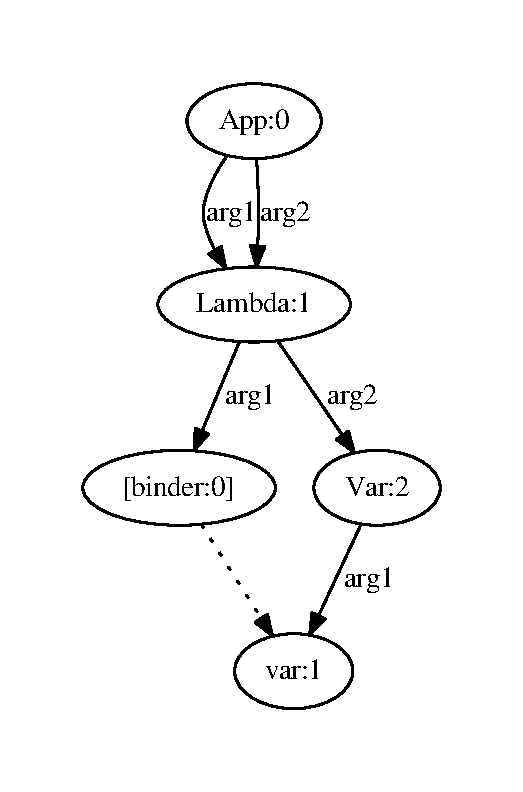
\includegraphics[scale=0.5]{pattern/pres_hash.pdf}
    \end{center}
  }
  
  \only<2>{
  
    \column{.5\textwidth}
    Sans hashconsing :
    \begin{center}
      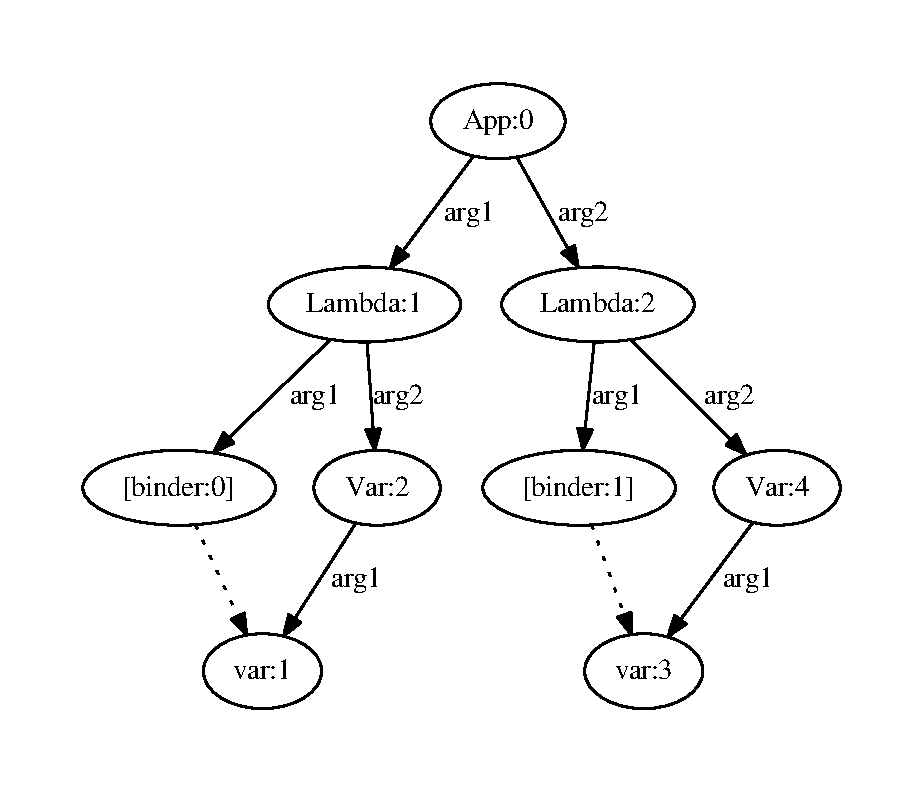
\includegraphics[scale=0.4]{pattern/no_hash.pdf}
    \end{center}
  }
\end{columns}
\end{frame}
